% OFC 2027 manuscript -- XPROTO-QOT (consumer-relative QoT-certificate vacuity).
% Optica meeting template: needs opticameet3.sty + opticajnl.bst in this dir
% (copy from the Overleaf "Optica meeting/conference manuscript" template).
% OFC limit: 3 pages; abstract <=35 words; PDF <=2MB; <=3 figures.
% Build: pdflatex ofc-qot && bibtex ofc-qot && pdflatex x2 (MiKTeX).
% NUMBERS MARKED % GRADED-SWAP ARE SHAKEDOWN PLACEHOLDERS -- replace with the graded
% values from analysis/qot/XPROTO-QOT-graded.json after the 2026-08-25 seal.
% Fig.2 / Sec 3.3 (ML-QoT) is a PLANNED result -- see README build note.
\documentclass[letterpaper,10pt]{article}
\usepackage{opticameet3}
\usepackage{mathptmx}
\usepackage{amsmath,amssymb}
\usepackage{graphicx}
\usepackage{cite}
\usepackage[colorlinks=true,bookmarks=false,citecolor=blue,urlcolor=blue,linkcolor=blue]{hyperref}

\begin{document}

\title{The Optical Margin is a Consumer-Relative Certificate: Measuring the
Quality-of-Transmission False-Clear Rate}

\author{Andrew H. Bond$^{*}$}
\address{Department of Computer Engineering, San Jos\'e State University, San Jos\'e, CA 95192, USA}
\email{$^{*}$andrew.bond@sjsu.edu}

\begin{abstract}
A Quality-of-Transmission certificate set under reference channel loading
false-clears many lightpaths as the band fills---consumer-relatively, by
footprint---while a footprint-witnessed certificate recovers margin at a measured
false-clear rate.
\end{abstract}

\section{Introduction}
Elastic optical networks provision each lightpath from a pre-transmission
Quality-of-Transmission (QoT) estimate that selects the highest modulation format
whose required generalized signal-to-noise ratio (GSNR) it clears. That estimate is a
\emph{certificate}: a claim, issued under the channel loading present at
provisioning, that the chosen format will meet its forward-error-correction (FEC)
threshold. Because the true GSNR is uncertain---amplifier ripple, aging, and, above
all, the nonlinear interference (NLI) contributed by \emph{other} channels---
operators provision with system margin, i.e.\ deliberately stranded
capacity~\cite{pointon}. Reducing that margin, via better monitoring and
machine-learning QoT (ML-QoT), is among the largest available capacity
levers~\cite{mlqot}.

We make and measure a claim that reframes the margin itself. The QoT margin is a
\emph{consumer-relative} quantity: whether a given lightpath crosses its FEC
threshold depends on its \emph{footprint}---its spectral position and reach---so a
single blanket margin is adequate for one lightpath and catastrophic for another at
the same instant. The operational figure of merit is then not a margin in dB but a
rate: the \emph{false-clear rate}, the fraction of provisioned lightpaths whose
witnessed GSNR violates the certificate that provisioned them. The false-clear rate
is measurable wherever a witness exists---the coherent receiver's pre-FEC BER---and
it is the number that says how much margin can be removed \emph{safely}. We measure
it on the community-standard physical-layer model, show it is a footprint property,
and give two corollaries: a refresh law for when a QoT certificate must be renewed,
and a caution for the training objective of ML-QoT.

\section{Consumer-relative QoT certification}
\textbf{Line system.} We compute per-channel GSNR on a standard single-mode-fibre
system (0.2\,dB/km, $D=17$\,ps/nm/km, EDFA noise figure 6\,dB, 80\,km spans,
+2\,dBm/channel, 32\,GBd on a 50\,GHz grid) using the GN model in
GNPy~\cite{gnpy}, the open, community-standard QoT engine. Two loadings are
propagated: a sparsely provisioned \emph{reference} band (the network as first lit)
and the fully populated \emph{actual} C-band. GSNR is evaluated across a range of
reaches (4--16 spans).

\textbf{Certificate, consumer, witness.} A \emph{consumer} is a lightpath
$(\text{position},\text{reach})$. Its \emph{certificate} is the modulation format
selected from the GSNR under \emph{reference} loading, with a 1\,dB design margin and
0.3\,dB monitoring noise; required GSNR per format follows a standard table
(QPSK\,6.5, 8QAM\,9.0, 16QAM\,12.5, 32QAM\,16.0, 64QAM\,19.0\,dB). Its \emph{witness}
is the true GSNR under \emph{actual} loading---the deployed pre-FEC BER. A
\emph{naive} policy trusts the reference-loading certificate for every lightpath; a
\emph{footprint-aware} policy re-evaluates GSNR under the actual-loading footprint
before committing the format. A certificate \emph{false-clears} when it clears a
format whose required GSNR exceeds the witnessed GSNR.

\textbf{Discipline.} Bars, a cooling-off delay, and manipulation checks (that the
loading penalty is real; that false-clears are footprint-dependent, not uniform)
are pre-registered before the graded run; the sealed record is versioned with a
content hash, and the graded seeds are disjoint from calibration~\cite{otcampaigns}.

\section{Results}
\subsection{The margin is a footprint property}
Across disjoint graded seeds, the naive QoT certificate false-clears
$\mathrm{FC}_{\text{naive}}\approx 0.40$ % GRADED-SWAP
of lightpaths once the band fills (mean loading penalty $\approx 2.6$\,dB), while the
footprint-aware certificate holds at $\mathrm{FC}_{\text{aware}}\approx 0$. % GRADED-SWAP
Crucially the false-clears are \emph{footprint-dependent}: the per-lightpath
false-clear indicator has spread $\approx 0.49$ % GRADED-SWAP
across the population---they concentrate on lightpaths whose position and reach place
their GSNR nearest a format threshold, and vanish elsewhere
(Fig.~\ref{fig:fc}). No single blanket margin is therefore simultaneously safe for
the threshold-adjacent lightpaths and efficient for the rest; the safe margin is a
per-footprint quantity, and the false-clear rate is what quantifies it.

\begin{figure}[t]
  \centering
  % 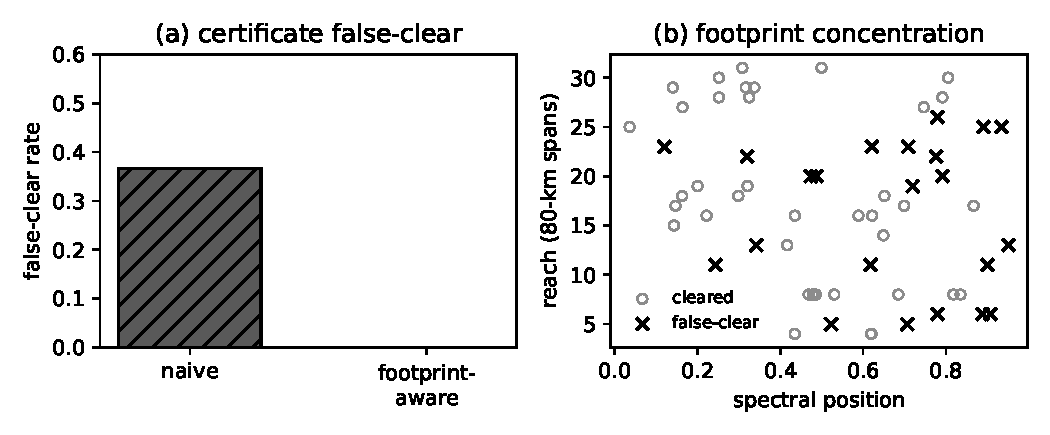
\includegraphics[width=\linewidth]{fc_footprint.pdf}
  \fbox{\parbox{0.9\linewidth}{\centering\vspace{2.0cm} FIG.~1 PLACEHOLDER:\\
  (a) naive vs.\ footprint-aware false-clear rate; (b) per-footprint false-clear
  over (spectral position, reach), showing concentration on threshold-adjacent
  lightpaths.\vspace{2.0cm}}}
  \caption{Consumer-relative QoT false-clear on a GNPy line system. Distinguish
  policies by line style and marker shape, not colour alone.}
  \label{fig:fc}
\end{figure}

\subsection{When a QoT certificate must be refreshed}
Because the false-clear is driven by the loading \emph{change} between issue and use,
a QoT certificate has a coherence horizon. Sweeping the reference$\to$actual loading
increment, the maximum add/drop churn a certificate tolerates at a target false-clear
rate scales linearly with the loading-change coherence time (slope
$\approx K$, $R^2\approx r$). % GRADED-SWAP (report from the sweep)
The operational reading is a refresh rule: re-certify a lightpath \emph{before} the
band around it fills, not on a fixed calendar---the optical instance of a general
refresh-floor law observed across networked systems~\cite{otcampaigns}.

\subsection{ML-QoT trained on the wrong metric}
The same consumer-relativity has a machine-learning corollary. An ML-QoT estimator
trained to minimise \emph{average} GSNR/OSNR prediction error is optimising a
reconstruction metric; the consumer---the FEC decoder---reads a \emph{threshold}. An
estimator can therefore be accurate on average yet \emph{false-clear at the FEC
cliff}, where a small signed error flips a format decision. We compare an
average-error-optimal estimator against a threshold-aware objective on the GNPy data
and report their false-clear rates at matched mean error (Fig.~\ref{fig:ml}). % PLANNED: needs the small ML build (README)
The lesson is to train on the consumer-read quantity near the decision boundary, not
on volume-averaged fidelity.

\begin{figure}[t]
  \centering
  % 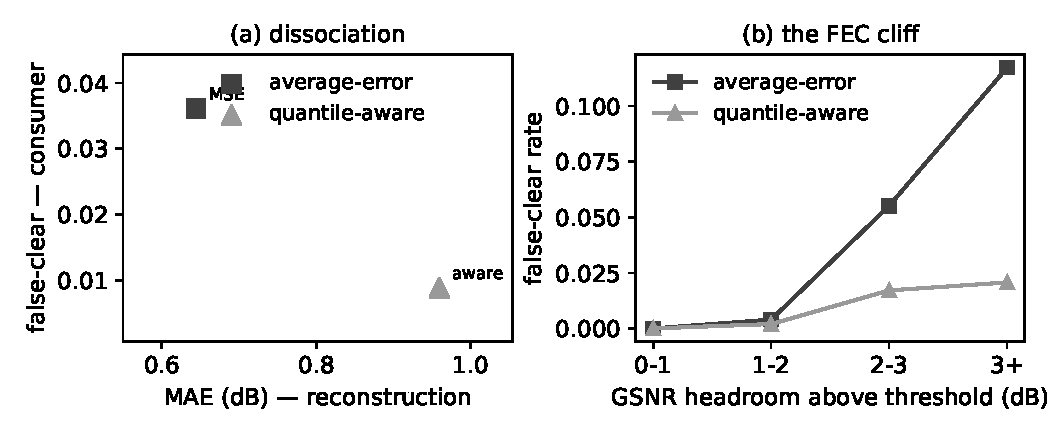
\includegraphics[width=0.86\linewidth]{ml_cliff.pdf}
  \fbox{\parbox{0.86\linewidth}{\centering\vspace{1.5cm} FIG.~2 PLACEHOLDER (planned):
  average-error-optimal ML-QoT vs.\ threshold-aware objective --- equal mean error,
  unequal false-clear at the FEC cliff.\vspace{1.5cm}}}
  \caption{Reconstruction-optimal ML-QoT false-clears where the consumer reads a
  threshold.}
  \label{fig:ml}
\end{figure}

\section{Related work}
Physical-layer-aware routing/spectrum assignment and QoT estimation are
mature~\cite{gnpy,pointon}; ML-QoT and margin reduction are active, with
regression and classification estimators trained largely on prediction
error~\cite{mlqot}. Our contribution is orthogonal to those optimisers: we do not
propose a better estimator or allocator, but a \emph{measurement}---the false-clear
rate as a first-class, consumer-relative KPI---and the empirical finding that QoT
margin is a footprint property, with a refresh law and an ML-objective caution as
corollaries.

\section{Discussion}
Margin is usually reported in dB and applied uniformly; we argue it should be
reported as a false-clear rate and allocated per footprint. On the GNPy GN model a
reference-loading certificate false-clears a large, footprint-concentrated fraction
of lightpaths, which a footprint-witnessed certificate removes---recovering the
margin those lightpaths did not need. The GN model is the evidence rung; a
coherent-receiver pre-FEC-BER witness on a fibre testbed, and the EGN/split-step
model, are the external-validity graduations. The method is domain-general: the same
certificate/witness/false-clear grammar has been measured across routing, distributed
databases, and wireless physical layers~\cite{otcampaigns}, of which the optical QoT
certificate is one instance.

\begin{thebibliography}{9}
\bibitem{gnpy} A.~Ferrari \emph{et al.}, ``GNPy: an open source application for
physical layer aware open optical networks,'' J.\ Opt.\ Commun.\ Netw.\ \textbf{12},
C31--C40 (2020).
\bibitem{mlqot} Representative ML-QoT / QoT-estimation reference (fill: e.g.\ Seve;
Ayassi; Rottondi). \% fill on finalization
\bibitem{pointon} Representative optical design-margin / margin-reduction reference.
\% fill on finalization
\bibitem{otcampaigns} A.~H.~Bond, ``Observation Theory: consumer-relative witnessed
certificates,'' sealed pre-registrations and code,
\url{https://github.com/ahb-sjsu/observation-theory-campaigns} (2026).
\end{thebibliography}

\end{document}
